\noindent\null
\begin{tikzpicture}[remember picture, overlay]
    % 4 đường kẻ ngang trang trí màu cyan ở góc trên lề trái
    \foreach \yy in {60, 64, 68, 72} {
        \draw[stewartcyan, line width=0.9pt] 
            ([xshift=14pt, yshift=-\yy pt]current page.north west) -- 
            ([xshift=48pt, yshift=-\yy pt]current page.north west);
    }

    % Ảnh minh họa mở đầu chương (tràn lề phải và đỉnh trang)
    \node[anchor=north west, inner sep=0pt] 
        at ([xshift=54pt, yshift=0pt]current page.north west) {
        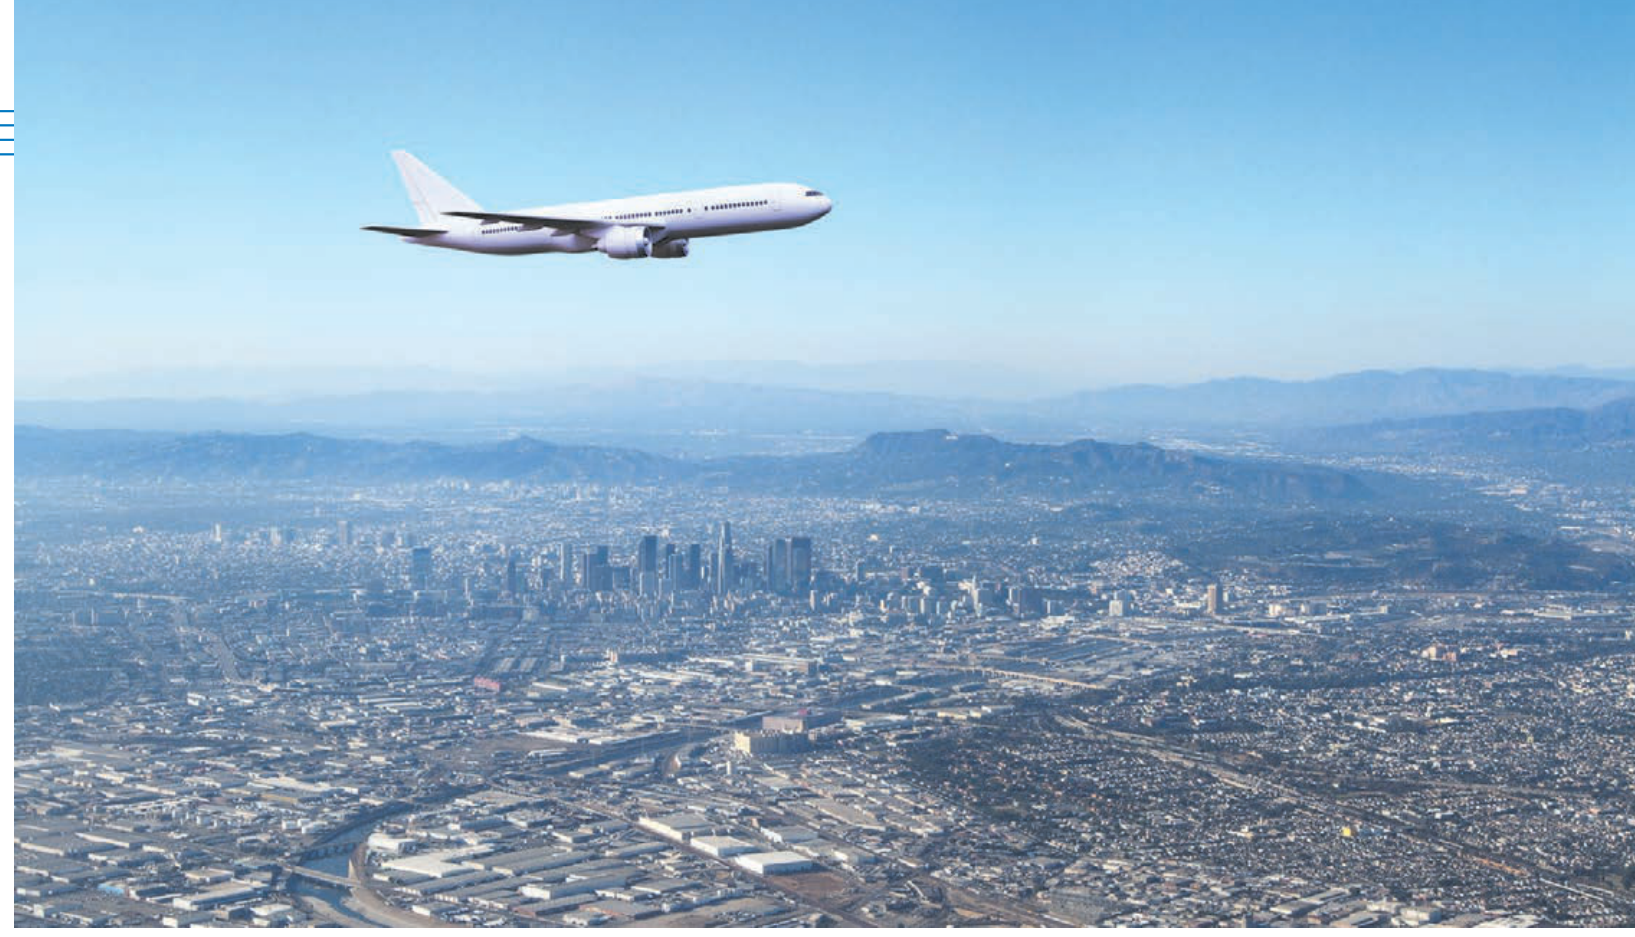
\includegraphics[width=558pt, height=308pt]{images/p0208_fig1.png}
    };

    % Chú thích dự án ứng dụng thực tế dưới ảnh
    \node[anchor=north west, inner sep=0pt, text width=440pt] 
        at ([xshift=54pt, yshift=-313.3pt]current page.north west) {
        {\fontsize{8.5}{11.5}\selectfont\sffamily\bfseries\color{stewartdarkgray}
        Trong dự án sau \textbf{\textsf{Mục 3.4}}, bạn sẽ tính khoảng cách từ đường băng sân bay mà tại đó một phi công nên bắt đầu hạ độ cao để có một cú tiếp đất êm ái.\par}
    };

    % Tác quyền ảnh
    \node[anchor=north west, inner sep=0pt] 
        at ([xshift=54pt, yshift=-337.5pt]current page.north west) {
        {\fontsize{7}{9}\selectfont\sffamily\color{stewartlightgray}Who is Danny / Shutterstock.com}
    };

    % Số thứ tự chương (Số 3 lớn màu cyan)
    \node[anchor=north east, inner sep=0pt] 
        at ([xshift=141pt, yshift=-365.8pt]current page.north west) {
        {\fontsize{82}{82}\selectfont\sffamily\bfseries\color{stewartcyan}3}
    };

    % Đường kẻ dọc màu cyan đặc trưng phân tách số chương và tiêu đề
    \draw[stewartcyan, line width=1.4pt] 
        ([xshift=148pt, yshift=-364pt]current page.north west) -- 
        ([xshift=148pt, yshift=-730pt]current page.north west);

    % Tiêu đề chương
    \node[anchor=north west, inner sep=0pt] 
        at ([xshift=158pt, yshift=-374pt]current page.north west) {
        {\fontsize{26}{32}\selectfont\sffamily\bfseries\color{black}Các quy tắc tính đạo hàm}
    };

    % Đoạn văn mở đầu chương
    \node[anchor=north west, inner sep=0pt, text width=322pt, align=justify] 
        at ([xshift=158pt, yshift=-459.1pt]current page.north west) {
        {\fontsize{9.5}{13.8}\selectfont
        \noindent\textbf{\textsf{CHÚNG TA ĐÃ THẤY CÁCH DIỄN GIẢI}} đạo hàm như hệ số góc và tốc độ thay đổi. Chúng ta đã sử dụng định nghĩa của đạo hàm để tính đạo hàm của các hàm số cho bởi công thức. Nhưng sẽ rất dài dòng và phức tạp nếu chúng ta luôn phải sử dụng định nghĩa, vì vậy trong chương này chúng ta phát triển các quy tắc để tìm đạo hàm mà không cần dùng trực tiếp định nghĩa. Các quy tắc tính đạo hàm này cho phép chúng ta tính toán tương đối dễ dàng đạo hàm của các đa thức, hàm phân thức hữu tỉ, hàm đại số, hàm mũ và hàm logarit, cũng như các hàm lượng giác và hàm lượng giác ngược. Sau đó, chúng ta sử dụng các quy tắc này để giải quyết các bài toán liên quan đến tốc độ thay đổi và sự xấp xỉ hàm số.\par}
    };

    % Số trang 173 ở góc dưới bên phải cột văn bản chính
    \node[anchor=north east, inner sep=0pt] 
        at ([xshift=480pt, yshift=-675.1pt]current page.north west) {
        {\fontsize{11}{13}\selectfont\sffamily\bfseries 173}
    };
\end{tikzpicture}
